\chapter{Exemple d'application}
\label{chap:application}%

On considère un échantillon $S_1$ formé de l'ensemble des prix
$S_1(t)$ à la fermeture du titre Abbey National entre le 31 juillet et
le 8 octobre 1991. La table \ref{prixabbeyn} présente l'ensemble des 50
observations. Cet échantillon a notamment été étudié précédemment par
\cite{buckle1995bayesian}.

\section{Description des données}
\label{sec:analysepA}

On évalue tout d'abord les rendements quotidiens $R_1$ à l'aide de
l'équation \eqref{eq:rendementlogprix}. On obtient alors 49
observations du processus des rendements $R(t)$, que l'on présente à
la figure \ref{fig:seriechronoR1} sous forme de série chronologique.

\begin{figure}[!ht]
  \centering
  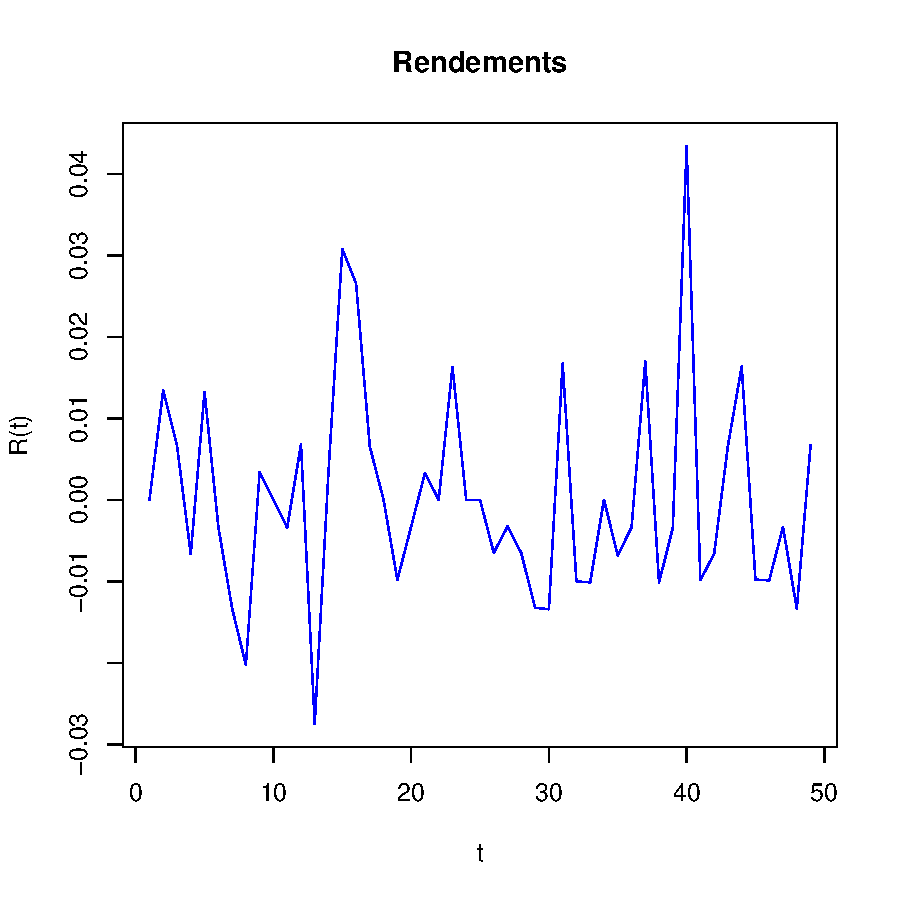
\includegraphics[height=4in,
  width=4in]{../graphiques/ABBEYN-chronologie.pdf}
  \caption{Représentation en série chronologique de l'échantillon
    $R_1$}
  \label{fig:seriechronoR1}
\end{figure}

On énumère d'abord quelques propriétés de cet échantillon qui pourront
compléter l'analyse. À la table \ref{tab:statordreR1}, on présente
quelques statistiques d'ordre. De plus, à la table
\ref{tab:statmomentsR1}, on retrouve quelques valeurs relatives aux
premiers moments.

\begin{table}[!ht]
  \centering
  \begin{tabular}{cccccc}
    \hline
    \textbf{Statistique d'ordre} & \textbf{Valeur} \\
    \hline
    Minimum & -0.027500\\ 
    1er quartile & -0.009790\\ 
    Médiane & -0.003260\\ 
    3e Quartile & 0.006620\\ 
    Maximum & 0.043400\\ 
    \hline
    
  \end{tabular}
  \caption{Statistiques d'ordre de l'échantillon $R_1$}
  \label{tab:statordreR1}
\end{table}

\begin{table}[!ht]
  \centering
  \begin{tabular}{cccc}
    \hline
    \textbf{Statistique} & \textbf{Valeur} \\
    \hline
    Moyenne & 0.000206\\ 
    Variance & 0.000169\\ 
    Coefficient d'asymétrie & 0.977563\\ 
    Coefficient d'aplatissement & 4.597114 \\ 
    \hline
  \end{tabular}
  \caption{Valeurs relatives aux premiers moments de l'échantillon $R_1$}
  \label{tab:statmomentsR1}
\end{table}

On présente maintenant la distribution des rendements sous la forme
d'une courbe de densité à la figure \ref{fig:distributionR1}.

\begin{figure}[!ht]
  \centering
  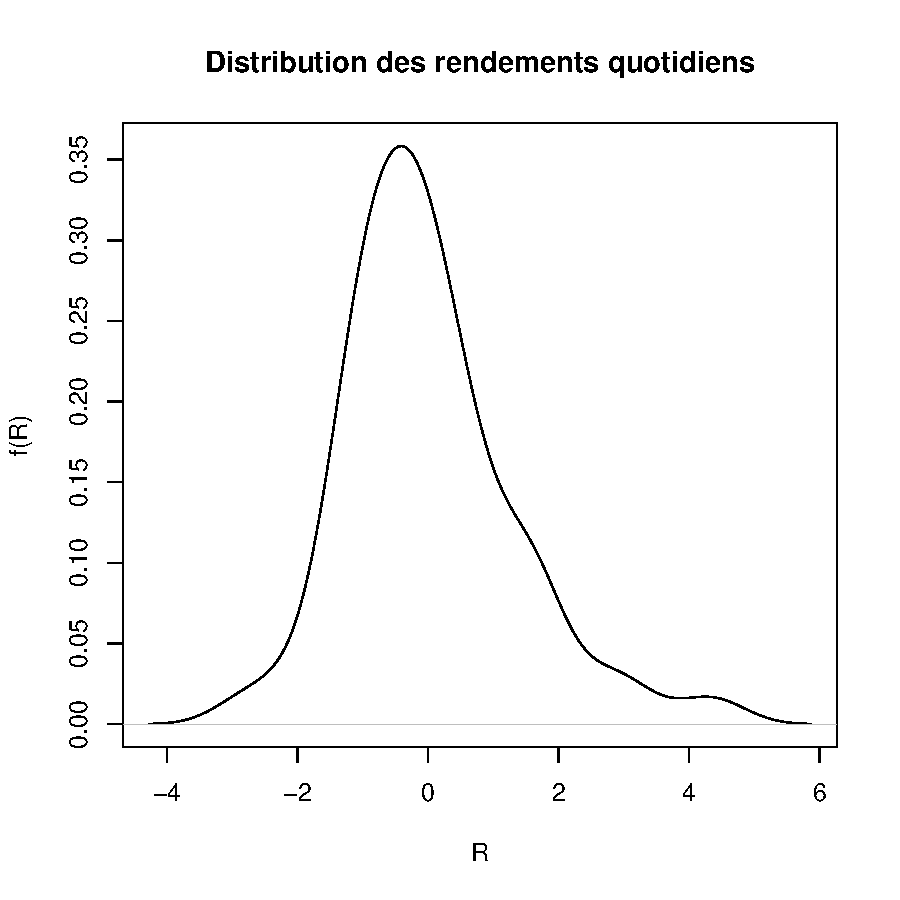
\includegraphics[height=4in,width=4in]{../graphiques/ABBEYN-histogramme.pdf}
  \caption{Distribution de la variable aléatoire $R_1$}
  \label{fig:distributionR1}
\end{figure}

À l'aide du test de normalité d'Epps-Pulley (Section
\ref{sec:test-de-epps}), on vérifie si la distribution des rendements
$R_1$ est significativement différente de la normale. On fixe le seuil
de tolérance $\alpha = 5\% $.

On évalue d'abord la statistique $EP_T$
\eqref{eq:statistiqueEppsPulley}, puis la statistique modifiée
$EP_T^{*}$ \eqref{eq:EppsPulleyMod} étant donné que $T>10$. La table
\ref{tab:eppspulleyR1} présente les résultats.

\begin{table}[!ht]
  \centering
  \begin{tabular}{ll}
    \hline
    \textbf{Statistique} & \textbf{Valeur} \\
    \hline
    $EP_T$ & 0.626033 \\
    $EP_T^{*}$ & 0.635568 \\
    $Z_T$ & 2.44824 \\
    $p$ & 0.007178 \\
    \hline
  \end{tabular}
  \caption{Test de normalité d'Epps-Pulley pour $R_1$}
  \label{tab:eppspulleyR1}
\end{table}

Étant donné que la valeur $p$ est inférieure au seuil $\alpha$, on
rejette l'hypothèse de normalité de l'échantillon $R_1$. On peut
vérifier cette affirmation à l'aide du graphique de comparaison des
quantiles empiriques avec ceux de la loi normale présenté à la figure
\ref{fig:qqplotR1}.

\begin{figure}[!ht]
  \centering
  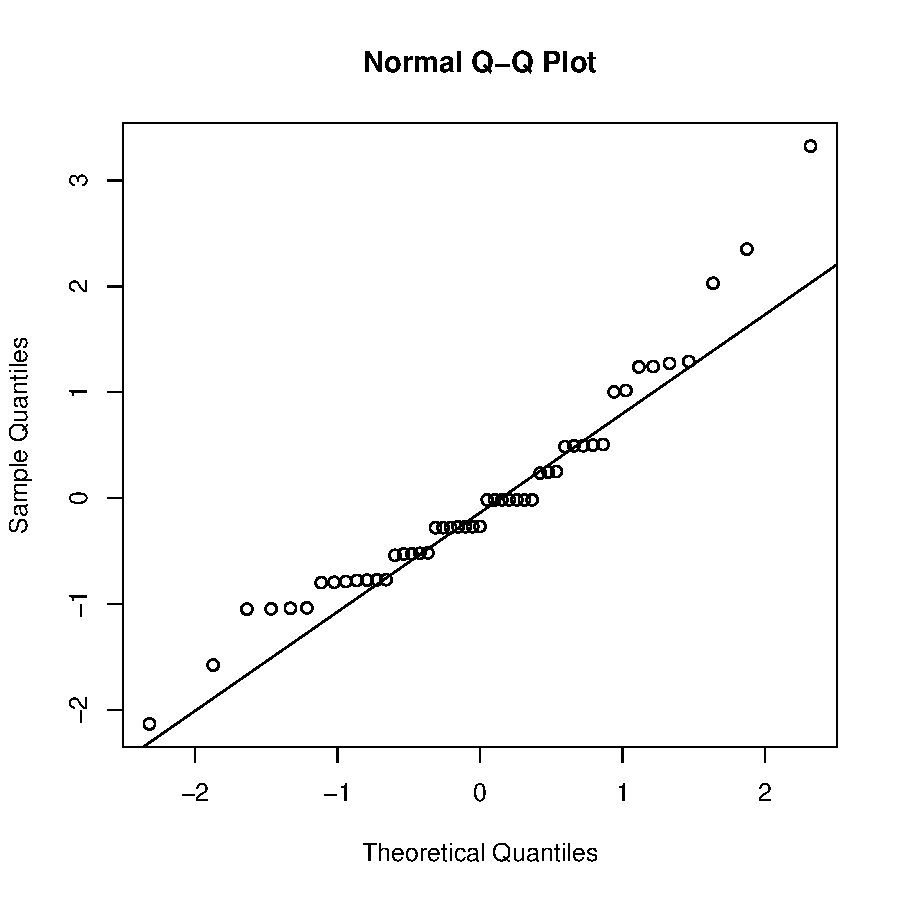
\includegraphics[height=4in,
  width=4in]{../graphiques/ABBEYN-qq.pdf}
  \caption{Graphique Quantile-Quantile}
  \label{fig:qqplotR1}
\end{figure}

\section{Estimation}
\label{sec:estimation}

Dans cette section, on estime les paramètres de la distribution de
Laplace asymétrique généralisée pour l'échantillon de données centrées
et réduites $R_1^{*}$, à l'aide des méthodes:
\begin{itemize}
\item des moments généralisée itérative (Section \ref{sec:GMMtwostep})
\item d'estimation gaussienne de Whittle (table
  \ref{tab:methodesquad})
\item de l'équation d'estimation optimale de Crowder (Section
  \ref{sec:equationsquadopt}) et
\item de l'équation d'estimation optimale modifiée (Section
  \ref{sec:eqoptmodif}).
\end{itemize}

On évalue d'abord le vecteur de paramètres initiaux $\theta_0$ à
l'aide des équations \eqref{eq:ptdepartGAL}. On effectue ensuite une
première optimisation à l'aide de chacune des trois méthodes afin de
pouvoir évaluer la matrice de pondération qui servira à la seconde. La
table \ref{tab:premiereoptimR1} présente les paramètres obtenus
$\theta_1$.

\begin{table}[!ht]
  \centering
  \begin{tabular}{lcccc}
    \hline
    \textbf{Méthode} & $\theta$ & $\sigma$ & $\mu$ & $\tau$ \\
    \hline
    Paramètres initiaux & -0.612081 & 0.515932 & 0.325854 & 1.878388 \\
    \hline
    Moments généralisée & -0.641646 & 0.625908 & 0.326366 & 1.965995 \\
    Estimation gaussienne & -0.776204 & 0.581154 & 0.385120 & 2.015437 \\
    Équation d'estimation optimale & -0.660300 & 0.645678 & 0.376654 & 1.753069 \\
    Équation d'estimation optimale modifiée & -0.711439 & 0.606642 & 0.362932 & 1.960299 \\
    \hline
  \end{tabular}
  \caption{Paramètres $\theta_1$ de la première optimisation}
  \label{tab:premiereoptimR1}
\end{table}

On obtient la matrice de variance-covariance des paramètres pour les
méthodes basées sur une équation d'estimation
\eqref{eq:VarAsymptEstEE} en évaluant l'inverse de la
variance-covariance des éléments composant celle-ci
\eqref{eq:Crowder86-th3.3-def-2} et le gradient
\eqref{eq:Crowder86-th3.3-def-1}:
\begin{itemize}
\item Pour la méthode d'estimation gaussienne:
  \begin{align}
    \label{eq:vcov1gaussR1}
    \mathbf{S}_T^{*}(\hat\theta_1;R_1^{*}) = \begin{bmatrix}
      1.13756e-03 &-0.00207546& 0.000917316& 7.46064e-06\\
      -2.07546e-03 & 0.00984423& 0.002340623& 1.24328e-03\\
      9.17316e-04 & 0.00234062& 0.003399880& 8.38932e-04\\
      7.46064e-06 & 0.00124328& 0.000838932& 2.60840e-04
    \end{bmatrix}
  \end{align}
\item Pour la méthode de l'équation d'estimation optimale:
  \begin{align}
    \label{eq:vcov1eeR1}
    \mathbf{S}_T^{*}(\hat\theta_1;R_1^{*}) = \begin{bmatrix}
      1.47029e-03 &-0.00212833& 0.00133597& 2.84688e-05\\
      -2.12833e-03 & 0.01115599& 0.00277669& 1.95192e-03\\
      1.33597e-03 & 0.00277669& 0.00396182& 1.18855e-03\\
      2.84688e-05 & 0.00195192& 0.00118855& 4.92502e-04
    \end{bmatrix}
  \end{align}
\item Pour la méthode de l'équation d'estimation optimale modifiée:
  \begin{align}
    \label{eq:vcov1eemodR1}
    \mathbf{S}_T^{*}(\hat\theta_1;R_1^{*}) = \begin{bmatrix}
      1.03165e-03& -0.00146603& 0.001145269& 6.63861e-05\\
      -1.46603e-03&  0.00812868& 0.001989247& 1.17588e-03\\
      1.14527e-03&  0.00198925& 0.003435163& 8.33622e-04\\
      6.63861e-05& 0.00117588& 0.000833622& 2.71162e-04
    \end{bmatrix}
  \end{align}
\end{itemize}

On peut ainsi construire des intervalles de confiance pour les
paramètres estimés. On utilise un seuil de tolérance de $\alpha=5\%$:
\begin{itemize}
\item Pour la méthode d'estimation gaussienne:\\ \\
  \begin{tabular}{rrrr}
    \hline
    & \textbf{Borne inférieure} & \textbf{Valeur estimée} & \textbf{Borne supérieure} \\
    \hline
    $\theta$ & -0.8328 & -0.7762 & -0.7197 \\ 
    $\sigma$ & 0.4148 & 0.5812 & 0.7475 \\ 
    $\mu$ & 0.2874 & 0.3851 & 0.4829 \\ 
    $\tau$ & 1.9884 & 2.0154 & 2.0425 \\ 
    \hline
  \end{tabular}\\

\item Pour la méthode de l'équation d'estimation optimale:\\ \\
  \begin{tabular}{rrrr}
    \hline
    & \textbf{Borne inférieure} & \textbf{Valeur estimée} & \textbf{Borne supérieure} \\
    \hline
    $\theta$ & -0.7246 & -0.6603 & -0.5960 \\ 
    $\sigma$ & 0.4686 & 0.6457 & 0.8228 \\ 
    $\mu$ & 0.2711 & 0.3767 & 0.4822 \\ 
    $\tau$ & 1.7159 & 1.7531 & 1.7903 \\ 
    \hline
  \end{tabular}\\

\item Pour la méthode de l'équation d'estimation optimale modifiée:\\ \\
\begin{tabular}{rrrr}
  \hline 
  & \textbf{Borne inférieure} & \textbf{Valeur estimée} & \textbf{Borne supérieure} \\ 
  \hline
  $\theta$ & -0.7653 & -0.7114 & -0.6576 \\ 
  $\sigma$ & 0.4555 & 0.6066 & 0.7578 \\ 
  $\mu$ & 0.2647 & 0.3629 & 0.4612 \\ 
  $\tau$ & 1.9327 & 1.9603 & 1.9879 \\ 
  \hline
\end{tabular}\\

\end{itemize}

À l'aide de l'inverse de la variance-covariance des conditions de
moments et des équations d'estimation, on peut effectuer une seconde
optimisation afin d'obtenir des estimateurs convergents. Pour la
méthode des moments généralisée, on utilisera plutôt une procédure
itérative. Les paramètres présentés à la table
\ref{tab:secondeoptimR1} sont donc ceux obtenus avec la convergence de
l'algorithme itératif de la section \ref{sec:GMMtwostep} avec un
critère d'arrêt $\epsilon=10^{-7}$ \eqref{eq:criterearret}.

\begin{table}[!ht]
  \centering
  \begin{tabular}{lcccc}
    \hline
    \textbf{Méthode} & $\theta$ & $\sigma$ & $\mu$ & $\tau$ \\
    \hline
    Moments généralisée & -0.640067 & 0.625431 & 0.324311 & 1.973623 \\
    Estimation gaussienne & -0.775071 & 0.581413 & 0.384342 & 2.016619 \\
    Équation d'estimation optimale & -0.658697 & 0.646516 & 0.376251 & 1.750685  \\
    Équation d'estimation optimale modifiée & -0.712450 & 0.606193 & 0.363196 & 1.961614  \\
    \hline
  \end{tabular}
  \caption{Paramètres $\theta_1$ de la première optimisation}
  \label{tab:secondeoptimR1}
\end{table}

Pour la méthode des moments généralisée, puisque l'on utilise une
procédure itérative, présenter la première matrice de
variance-covariance des paramètres n'est pas pertinent. On obtient
celle à la convergence de l'algorithme \eqref{matricevcovparamGMMnc}
en évaluant l'inverse de la variance-covariance des conditions de
moments \eqref{eq:matponderationproduith} et le gradient
\eqref{eq:gradientGMM}. On obtient donc:
\begin{align}
  \label{eq:vcov1gmmR1}
  \mathbf{S}_T^{*}(\hat\theta_{OPT};R_1^{*}) =
  \begin{bmatrix}
    0.00203708& 0.00438553& 0.00174636& 0.00154237\\
    0.00438553& 0.01207044& 0.00239640& 0.00384905\\
    0.00174636& 0.00239640& 0.00220402& 0.00104816\\
    0.00154237& 0.00384905& 0.00104816& 0.00127406
  \end{bmatrix}.
\end{align}

Pour les méthodes basées sur une équation d'estimation, on obtient,
pour la seconde optimisation, les variances-covariances suivantes:
\begin{itemize}
\item Pour la méthode d'estimation gaussienne:
  \begin{align}
    \label{eq:matvcov2R1-gauss}
    \mathbf{S}_T^{*}(\hat\theta_2;R_1^{*}) = \begin{bmatrix}
      1.13314e-03& -0.00206602& 0.000919367& 7.53773e-06\\
      -2.06602e-03 & 0.00983078& 0.002332240 &1.24238e-03\\
      9.19367e-04 & 0.00233224& 0.003395736& 8.36472e-04\\
      7.53773e-06 & 0.00124238& 0.000836472& 2.60254e-04
    \end{bmatrix}
  \end{align}
\item Pour la méthode de l'équation d'estimation optimale:
  \begin{align}
    \label{eq:matvcov2R1-ee}
    \mathbf{S}_T^{*}(\hat\theta_2;R_1^{*}) = \begin{bmatrix}
      1.47327e-03& -0.00212557& 0.00134221& 2.89119e-05\\
      -2.12557e-03 & 0.01116770 &0.00277803& 1.96072e-03\\
      1.34221e-03 & 0.00277803& 0.00396652& 1.19169e-03 \\
      2.89119e-05 & 0.00196072& 0.00119169& 4.95537e-04
    \end{bmatrix}
  \end{align}
\item Pour la méthode de l'équation d'estimation optimale modifiée:
  \begin{align}
    \label{eq:matvcov2R1-eemod}
    \mathbf{S}_T^{*}(\hat\theta_2;R_1^{*}) = \begin{bmatrix}
      1.03121e-03& -0.00146899& 0.001142696& 6.60715e-05\\
      -1.46899e-03 & 0.00812703 &0.001987649& 1.17298e-03\\
      1.14270e-03 & 0.00198765& 0.003432414& 8.32388e-04\\
      6.60715e-05 & 0.00117298& 0.000832388& 2.70299e-04
    \end{bmatrix}
  \end{align}
\end{itemize}

On peut donc construire des intervalles de confiance:
\begin{itemize}
\item Pour la méthode des moments généralisée:\\ \\
  \begin{tabular}{rrrr}
    \hline
    & \textbf{Borne inférieure} & \textbf{Valeur estimée} & \textbf{Borne supérieure} \\
    \hline
    $\theta$ &  -0.715736& -0.640067& -0.564397\\
    $\sigma$ & 0.441236 & 0.625431 & 0.809627\\
    $\mu$ & 0.245602 & 0.324311 & 0.403020\\
    $\tau$ & 1.913780 & 1.973623 & 2.033466\\
    \hline
  \end{tabular} \\
\item Pour la méthode d'estimation gaussienne:\\ \\
  \begin{tabular}{rrrr}
    \hline
    & \textbf{Borne inférieure} & \textbf{Valeur estimée} & \textbf{Borne supérieure} \\
    \hline
    $\theta$ & -0.8315 & -0.7751 & -0.7186 \\ 
    $\sigma$ & 0.4152 & 0.5814 & 0.7476 \\ 
    $\mu$ & 0.2866 & 0.3843 & 0.4820 \\ 
    $\tau$ & 1.9896 & 2.0166 & 2.0437 \\ 
    \hline
  \end{tabular} \\
\item Pour la méthode de l'équation d'estimation optimale:\\ \\
  \begin{tabular}{rrrr}
    \hline
    & \textbf{Borne inférieure} & \textbf{Valeur estimée} & \textbf{Borne supérieure} \\
    \hline
    $\theta$ & -0.7230 & -0.6587 & -0.5943 \\ 
    $\sigma$ & 0.4693 & 0.6465 & 0.8237 \\ 
    $\mu$ & 0.2707 & 0.3763 & 0.4818 \\ 
    $\tau$ & 1.7134 & 1.7507 & 1.7880 \\ 
    \hline
  \end{tabular} \\
\item Pour la méthode de l'équation d'estimation optimale modifiée:\\ \\
  \begin{tabular}{rrrr}
    \hline
    & \textbf{Borne inférieure} & \textbf{Valeur estimée} & \textbf{Borne supérieure} \\
    \hline
    $\theta$ & -0.7663 & -0.7124 & -0.6586 \\ 
    $\sigma$ & 0.4551 & 0.6062 & 0.7573 \\ 
    $\mu$ & 0.2650 & 0.3632 & 0.4614 \\ 
    $\tau$ & 1.9341 & 1.9616 & 1.9892 \\ 
    \hline
  \end{tabular} \\
\end{itemize}

En utilisant la propriété \eqref{eq:transparamGALNS}, on retrouve les
paramètres, correspondants aux données $R(t)= \sqrt{Var[R_1]} R^{*}(t)
+ E[R_1], t=1,\ldots,50$, présentés à la table
\ref{tab:parametresdonneesorigineR1}.

\begin{table}[!ht] \centering
  \begin{tabular}{lcccc}
    \hline
    \textbf{Méthode} & $\theta$ & $\sigma$ & $\mu$ & $\tau$ \\ 
    \hline
    Moments généralisée& -0.008119 & 0.008134 & 0.002983 & 1.973623 \\ 
    Estimation gaussienne& -0.009875 & 0.007562 & 0.003535 & 2.016619 \\   
    Équation d'estimation optimale& -0.008361 & 0.008409 & 0.003460 & 1.750685 \\ 
    Équation d'estimation optimale modifiée& -0.009060 & 0.007884 & 0.003340 & 1.961614 \\ 
    \hline
  \end{tabular}
  \caption{Paramètres des données $R_1$}
  \label{tab:parametresdonneesorigineR1}
\end{table}

\section{Approximation}
\label{sec:approximationR1}

On effectue l'approximation des fonctions de densité et de répartition
pour un ensemble de points $r \in
\left\{-0.03,-0.02,-0.01,0,0.01,0.02,0.03 \right\}$ à l'aide de la
méthode du point de selle. On utilise les paramètres obtenus par la
méthode des moments généralisée.

On résout d'abord l'équation du point de selle
\eqref{eq:saddlepoint}. On illustre graphiquement cette équation pour
$r=0.01$ à la figure \ref{fig:equationptselle0.01R1} :
\begin{figure}[!ht]
  \centering
  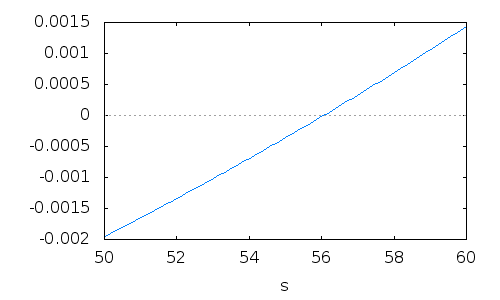
\includegraphics[scale=0.5]{../graphiques/pointdeselleGMM.png}
  \caption{Équation du point de selle pour $r=0.01$}
  \label{fig:equationptselle0.01R1}
\end{figure}

Le point de selle prend alors une valeur de $\hat{s}=56.050951$ dans
cette situation. En utilisant l'approximation de premier ordre
$\hat{f}_{R,1}(r)$
\eqref{eq:approximationsaddlepointordre1} % et celle
% de second ordre $\hat{f}_{R,2}(r)$
% \eqref{eq:approximationsaddlepointordre2}
de la fonction de densité, et en comparant le résutat avec la fonction
de densité ${f}_{R}(r)$ \eqref{eq:densitekotz2001}, on obtient les
résultats présentés à la table \ref{tab:approximationdensiteR1}. Dans
les deux cas, la fonction de densité a été normalisée à l'aide de
l'intégrale \eqref{eq:normalisationsaddle1}.

% latex table generated in R 2.15.2 by xtable 1.7-1 package Mon Aug 19
% 16:36:59 2013
\begin{table}[ht]
  \centering
  \begin{tabular}{cccc}
    & \multicolumn{2}{c}{\textbf{Densité}} & \multicolumn{1}{c}{\textbf{Erreur relative}} \\
    \hline
    $r$ & $\hat{f}_{R,1}(r)$ & ${f}_{R}(r)$ & $(\hat{f}_{R,1}(r)-{f}_{R}(r))/{{f}_{R}(r)}$ \\ 
    \hline
    -0.03 & 1.561365 & 2.065547 & -0.244091 \\ 
    -0.02 & 9.038616 & 10.702896 & -0.155498 \\ 
    -0.01 & 31.216317 & 37.581108 & -0.169361 \\ 
    0.00 & 33.015869 & 31.073988 & 0.062492 \\ 
    0.01 & 15.941633 & 12.450742 & 0.280376 \\ 
    0.02 & 5.988373 & 4.120017 & 0.453483 \\ 
    0.03 & 2.026838 & 1.246205 & 0.626409 \\ 
    \hline
  \end{tabular}
  \caption{Approximation de la densité de $R_1$}
  \label{tab:approximationdensiteR1}
\end{table}

On évalue ensuite la valeur de la fonction de répartition à l'aide de
l'approximation de premier ordre $\hat{F}_{R,1}(r)$
\eqref{eq:approximationsaddlepointREPordre1} % et de second ordre
% $\hat{F}_{R,2}(r)$ \eqref{eq:approximationsaddlepointREPordre2}
. On compare celle-ci à la valeur de la fonction de répartition
obtenue en intégrant numériquement la fonction de densité. Les
résultats sont présentés à la table \ref{tab:approximationrepartR1}.

% latex table generated in R 2.15.2 by xtable 1.7-1 package Mon Aug 19
% 16:49:26 2013
\begin{table}[ht]
  \centering
  \begin{tabular}{cccc}
    & \multicolumn{2}{c}{\textbf{Fonction de répartition}} & \multicolumn{1}{c}{\textbf{Erreur relative}} \\
    \hline
    $r$ & $\hat{F}_{R,1}(r)$ & ${F}_{R}(r)$ & $(\hat{F}_{R,1}(r)-{F}_{R}(r))/{{F}_{R}(r)}$ \\ 
    \hline
    -0.03 & 0.007402 & 0.011577 & -0.360606 \\ 
    -0.02 & 0.048942 & 0.064944 & -0.246402 \\ 
    -0.01 & 0.249911 & 0.292034 & -0.144241 \\ 
    0.00 & 0.625225 & 0.681167 & -0.082126 \\ 
    0.01 & 0.857830 & 0.889832 & -0.035965 \\ 
    0.02 & 0.951508 & 0.965916 & -0.014916 \\ 
    0.03 & 0.984393 & 0.990080 & -0.005744 \\
    \hline
  \end{tabular}
  \caption{Approximation de la fonction de répartition de $R_1$}
  \label{tab:approximationrepartR1}
\end{table}

\section{Graphiques}
\label{sec:graphiques}

On illustre graphiquement, aux figures \ref{fig:densite1R1} et
\ref{fig:densite3R1}, la fonction de densité de la distribution de
Laplace asymétrique généralisée avec les paramètres estimés par la
méthode des moments généralisée et la méthode de l'équation
d'estimation optimale. La table \ref{tab:courbesdensite} décrit
chacune des courbes.
\begin{table}[!ht]
  \centering
  \begin{tabular}{lp{12cm}}
    \hline
    \textbf{Abbréviation} & \textbf{Description} \\
    \hline
    Emp. & Données empiriques. \\
    Norm. & Densité de la distribution normale ayant les mêmes moyenne et variance que la variable aléatoire $R$. \\
    Estim. & Densité de la distribution de Laplace asymétrique généralisée avec les paramètres estimés.\\
    Pt selle o.1 & Approximation de premier ordre avec la méthode du point de selle. \\
    FFT & Transformée de Fourier rapide. \\
    \hline
  \end{tabular}
  \caption{Courbes de densité}
  \label{tab:courbesdensite}
\end{table}

On remarquera au passage que la méthode du point de selle nécessite
une normalisation. La valeur de l'intégrale $c$
\eqref{eq:normalisationsaddle1} pour les quatre méthodes se trouve à
la table \ref{tab:intapproxpointselleR1}.
\begin{table}[!ht]
  \centering
  \begin{tabular}{ll}
    \hline
    \textbf{Méthode} & \textbf{Valeur de l'intégrale $c$}\\
    \hline
    Moments généralisée & 0.920148 \\
    Estimation gaussienne & 0.932246 \\
    Équation d'estimation optimale & 0.917326 \\
    Équation d'estimation optimale modifiée & 0.925781 \\
    \hline
  \end{tabular}
  \caption{Valeur de l'intégrale de l'approximation de la densité par la méthode du point de selle }
  \label{tab:intapproxpointselleR1}
\end{table}

\begin{figure}[!ht]
  \centering
  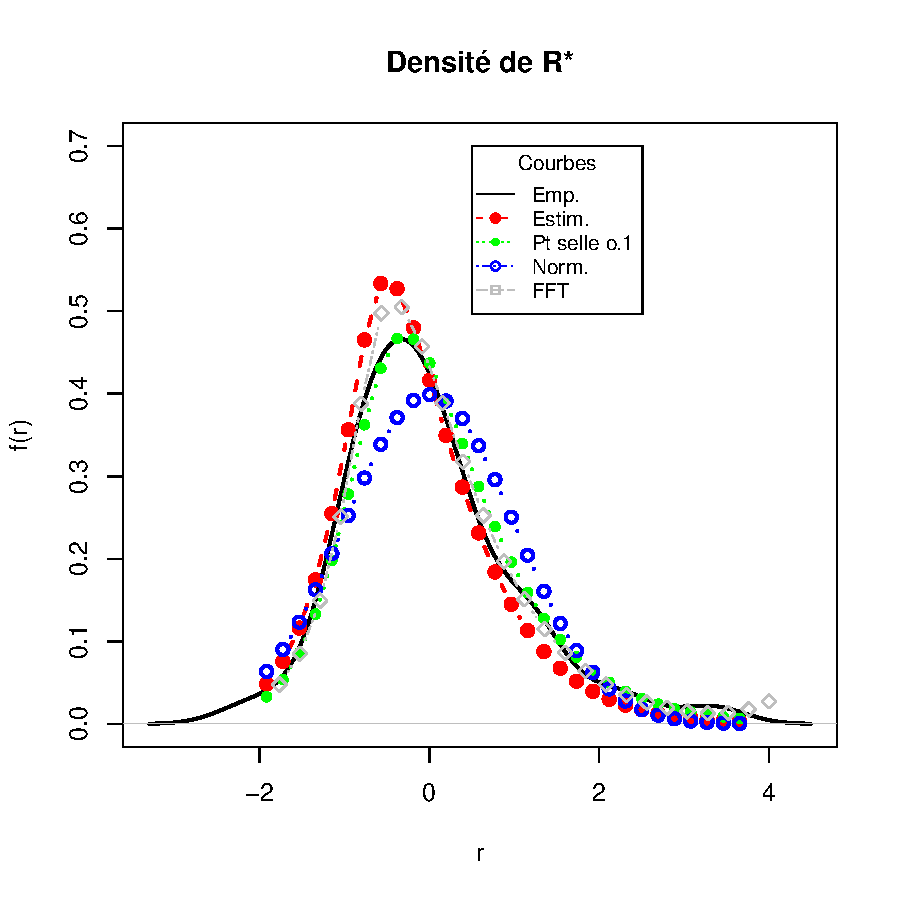
\includegraphics[height=6in,
  width=6in]{../graphiques/ABBEYN-densiteGALmu-7.pdf}
  \caption{Densité de $R_1^{*}$ selon la méthode des moments
    généralisée}
  \label{fig:densite1R1}
\end{figure}

\begin{figure}[!ht]
  \centering
  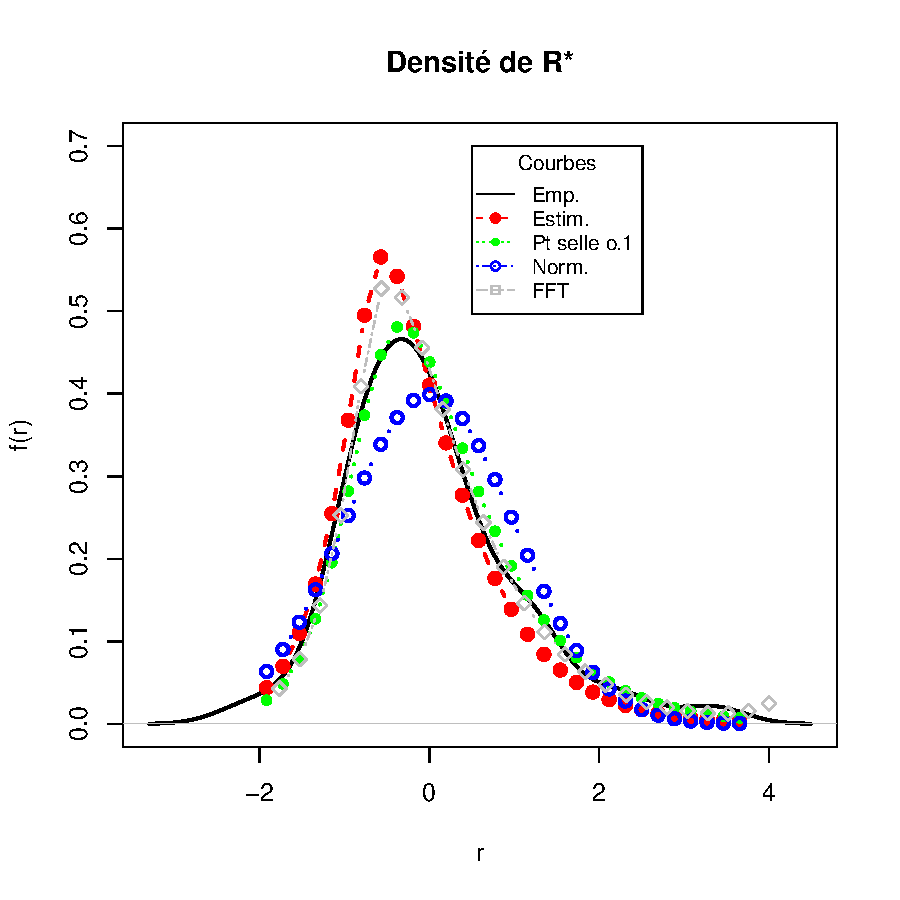
\includegraphics[height=6in,
  width=6in]{../graphiques/ABBEYN-densiteGALmu-5.pdf}
  \caption{Densité de $R_1^{*}$ selon la méthode de l'équation
    d'estimation optimale}
  \label{fig:densite3R1}
\end{figure}

\clearpage
\section{Tests statistiques}
\label{sec:tests-statistiques}

On effectue le test du $\chi^2$ en utilisant sept classes optimales
déterminées par l'algorithme du logiciel GNU R. On obtient la fonction
de répartition à partir de la fonction caractéristique en utilisant la
formule d'inversion \eqref{eq:approxinvfncaract}. On se rappelle que
cet algorithme produit surtout des erreurs aux extrémités de la
distribution. Par contre, ce test donne davantage d'importance aux
classes ayant un plus grand nombre de données par construction. On
utilisera donc l'inversion plutôt que la méthode du point de selle. On
obtient la statistique $Q_{6}$ présentée à la table
\ref{tab:testchi2R1} à partir de la définition \eqref{eq:statchi2}. On
utilise un seuil de tolérance $\alpha = 5\%$.
\begin{table}[!ht]
  \centering
  \begin{tabular}{ll}
    \hline
    \textbf{Méthode} & \textbf{Valeur de la statistique $Q_{6}$} \\
    \hline
    Moments généralisée              &  0.484919 \\
    Estimation gaussienne        &  0.473527 \\
    Équation d'estimation optimale    &  0.531888 \\
    Équation d'estimation optimale modifiée  &  0.494769 \\
    \hline
  \end{tabular}
  \caption{Test du $\chi^2$}
  \label{tab:testchi2R1}
\end{table}

Ce test ne permet pas de rejeter l'hypothèse de la distribution de
Laplace asymétrique généralisée avec les paramètres obtenus pour
aucune des méthodes d'estimation.

On effectue maintenant le test de Kolmogorov-Smirnov. Comme celui-ci
est basé sur la fonction de répartition, on utilisera la même méthode
que précédemment, impliquant l'inversion de la fonction
caractéristique. On évalue la fonction de répartition en chaque point
de l'échantillon $R_1^{*}$ et l'on obtient la statistique $D_{49}$
présentée à la table \ref{tab:testKSR1} à l'aide de la définition
\eqref{eq:statks}. En utilisant un seuil de tolérance de $\alpha=5\%$,
on obtient une valeur critique de $0.194286$.

\begin{table}[!ht]
  \centering
  \begin{tabular}{ll}
    \hline
    \textbf{Méthode} & \textbf{Valeur de la statistique $D_{49}$} \\
    \hline
    Moments généralisée & 0.0684329  \\
    Estimation gaussienne & 0.0784436   \\
    Équation d'estimation optimale & 0.0758317  \\
    Équation d'estimation optimale modifiée & 0.074668  \\
    \hline
  \end{tabular}
  \caption{Test de Kolmogorov-Smirnov}
  \label{tab:testKSR1}
\end{table}

Encore une fois, on ne peut pas rejeter l'hypothèse de la distribution
de Laplace asymétrique généralisée avec les paramètres estimés pour
chacune des méthodes.

Ces deux tests sont approximatifs, puisque les paramètres n'ont pas
été estimés en minimisant la statistique utilisée. Cependant, on
obtient un test asymptotiquement exact en utilisant une statistique de
distance minimale basée sur la fonction génératrice des moments, tel
que développé à la section \ref{sec:test-de-distance}. Avec un seuil
de tolérance de $\alpha=5\%$, on obtient une valeur critique de
67.5048. Les statistiques obtenues sont présentées à la table
\ref{tab:testDMR1}.

\begin{table}[!ht]
  \centering
  \begin{tabular}{ll}
    \hline
    \textbf{Méthode} & \textbf{Valeur de la statistique $Td(F_{49},F_{\theta})$} \\
    \hline
    Moments généralisée & 0.226891 \\
    Estimation gaussienne & 0.110573  \\
    Équation d'estimation optimale & 0.074020 \\
    Équation d'estimation optimale modifiée & 0.108625 \\
    \hline
  \end{tabular}
  \caption{Test de distance minimale basé sur la fonction génératrice des moments}
  \label{tab:testDMR1}
\end{table}

On ne peut pas rejeter l'hypothèse de la distribution de Laplace
asymétrique généralisée avec les paramètres estimés pour chacune des
méthodes avec ce test.

\section{Évaluation d'options}
\label{sec:evaluation-doptions}

À titre d'exemple, on évaluera une option européenne dont les
différentes caractéristiques figurent à la table
\ref{tab:caracteristiqueoptionR1}.

\begin{table}[!ht]
  \centering
  \begin{tabular}{ll}
    \hline
    \textbf{Caractéristique} & \textbf{Valeur} \\
    \hline
    Type & Option de vente \\
    Échéance ($T$) & 30 jours \\
    Valeur actuelle du titre ($S(0)$) & 299 \\
    Prix d'exercice ($K$) & entre 95\% et 105\% de la valeur actuelle \\
    Taux sans risque annuel ($r_f$) & 5\% \\
    \hline
  \end{tabular}
  \caption{Caractéristiques de l'option}
  \label{tab:caracteristiqueoptionR1}
\end{table}

À partir des paramètres de la table
\ref{tab:parametresdonneesorigineR1}, en utilisant l'équation
martingale appliquée à la distribution de Laplace asymétrique
généralisée \eqref{eq:martingaleGAL}, on obtient l'ensemble
correspondant pour la mesure neutre au risque. On rappelle que
celle-ci n'est pas unique étant donné que le processus de Laplace est
un processus de sauts. La table \ref{tab:paramrisqueneutreR1} présente
ces paramètres.
\begin{table}[!ht]
  \centering
  \begin{tabular}{lcccc}
    \hline
    & $\theta$ & $\sigma$ & $\mu$ & $\tau$ \\ 
    \hline
    Moments généralisée & -0.005824 & 0.008134 & 0.002983 & 1.973623 \\ 
    Estimation gaussienne & -0.007062 & 0.007562 & 0.003535 & 2.016619 \\ 
    Équation d'estimation optimale & -0.005993 & 0.008409 & 0.003460 & 1.750685 \\ 
    Équation d'estimation optimale modifiée & -0.006487 & 0.007884 & 0.003340 & 1.961614 \\ 
    \hline
  \end{tabular}
  \caption{Paramètres neutres au risque}
  \label{tab:paramrisqueneutreR1}
\end{table}

On présente les graphiques de la valeur du prix de l'option de vente
pour les méthodes des moments généralisée et de l'équation d'estimation
optimale aux figures \ref{fig:prix1R1-1} et \ref{fig:prix1R1-3}.  On
peut facilement remarquer le manque de précision de l'approche de
Carr-Madan, qui s'approche de la courbe de Black-Scholes lorsque le
titre est dans la monnaie et qui se met à osciller dès que le titre
est hors de la monnaie. Les méthodes de Epps et de Heston donnent des
résultats très similaires, et l'approximation du point de selle
d'ordre 1 est très précise dans ce contexte.
\begin{figure}[!ht]
  \centering
  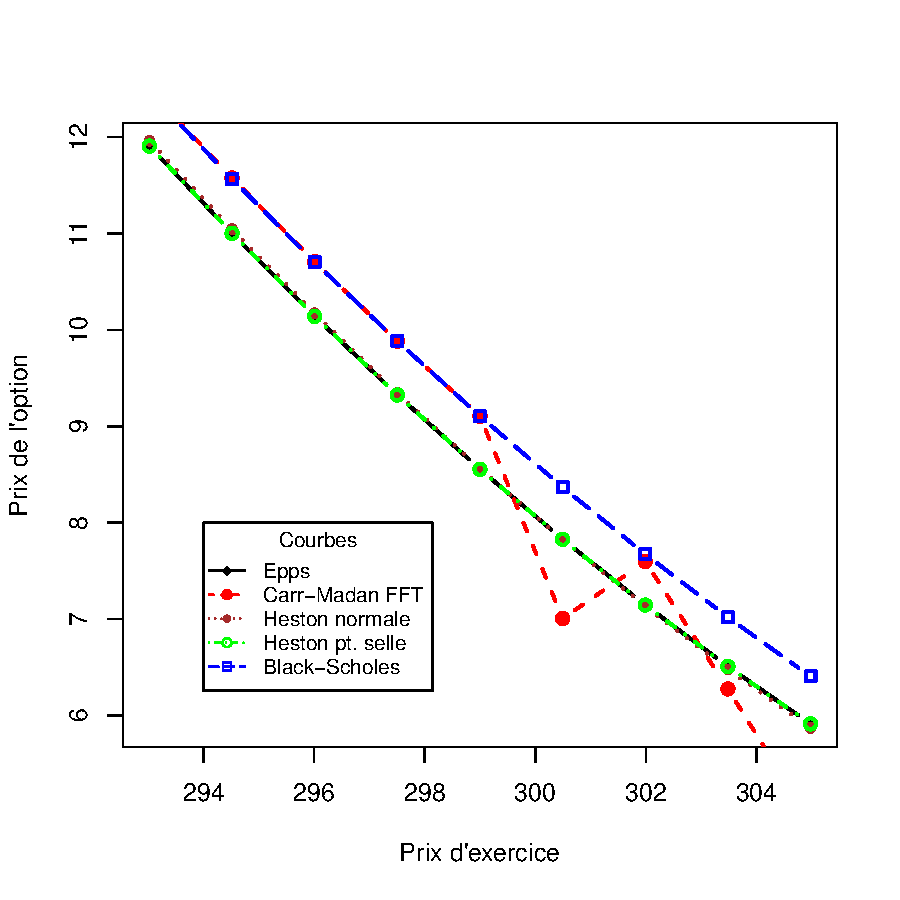
\includegraphics[height=6in,
  width=6in]{../graphiques/ABBEYN-callGAL-7.pdf}
  \caption{Prix de l'option selon les paramètres estimés avec la
    méthode des moments généralisée}
  \label{fig:prix1R1-1}
\end{figure}

\begin{figure}[!ht]
  \centering
  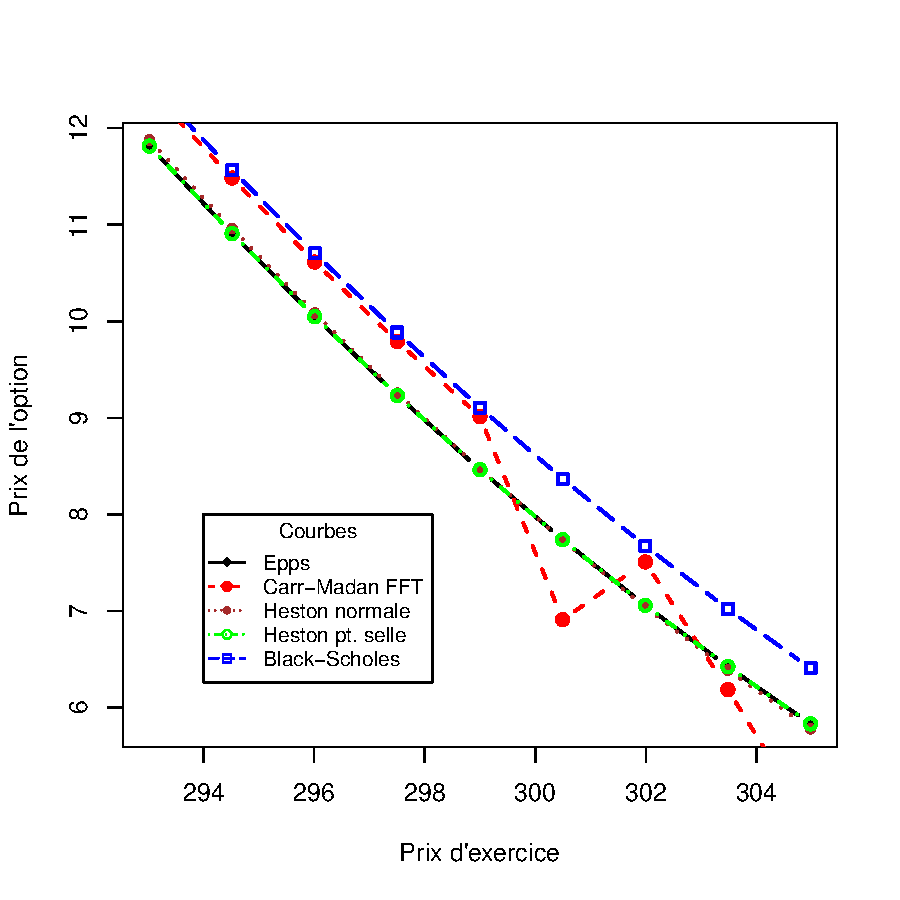
\includegraphics[height=6in,
  width=6in]{../graphiques/ABBEYN-callGAL-5.pdf}
  \caption{Prix de l'option selon les paramètres estimés avec la
    méthode de l'équation d'estimation optimale}
  \label{fig:prix1R1-3}
\end{figure}

%%% Local Variables: 
%%% mode: latex
%%% TeX-master: "gabarit-maitrise"
%%% End: 
